\documentclass[11pt, oneside]{article} 
\usepackage{geometry}
\geometry{letterpaper} 
\usepackage{graphicx}
	
\usepackage{amssymb}
\usepackage{amsmath}
\usepackage{parskip}
\usepackage{color}
\usepackage{hyperref}

\graphicspath{{/Users/telliott_admin/Dropbox/Tex/png/}}
% \begin{center} 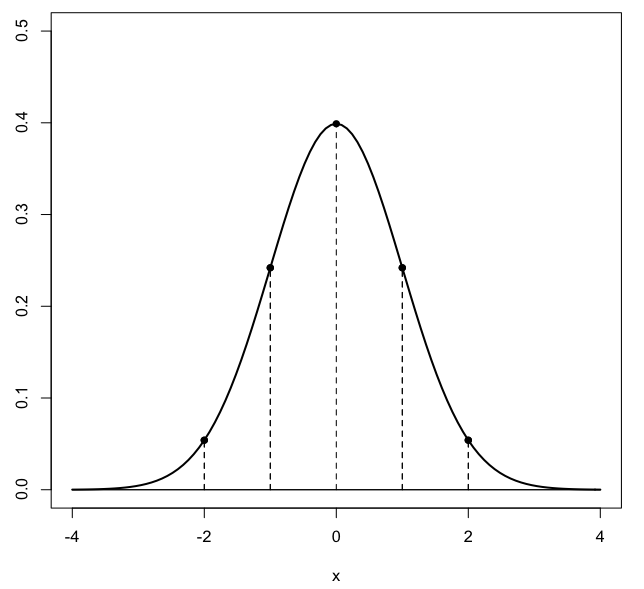
\includegraphics [scale=0.4] {gauss3.png} \end{center}

\title{Basic geometry and congruence of triangles}
\date{}

\begin{document}
\maketitle
\Large
From a previous chapter, Euclid's third postulate was:

$\circ$   Given any straight line segment, a circle can be drawn having the segment as radius and one endpoint as center.  The tool to do this is called a compass:

\url{https://en.wikipedia.org/wiki/Compass_(drawing_tool)}

If the radius is extended so that it cuts the circle at two points, it is called a diameter.  We saw previously that one can construct a line perpendicular to any given line.  If that line is constructed perpendicular to the diameter at the point where it meets the circle, the new line is called a tangent line.  By definition, the tangent line touches the circle at a single point.

\subsection*{arcs of a circle}

\begin{center} 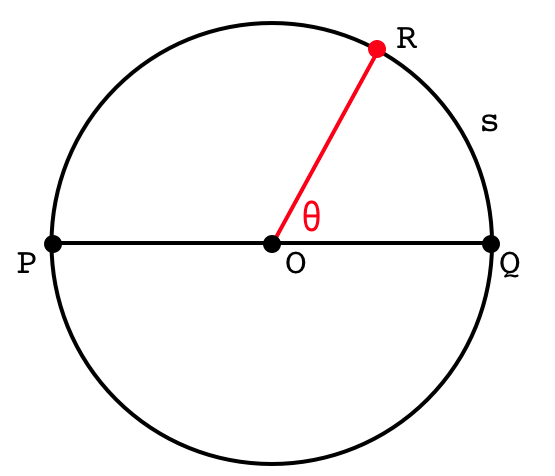
\includegraphics [scale=0.30] {arcs1.png} \end{center}
In calculus and analytical geometry angles are defined in terms of radians of arc. For a unit circle with radius = $1$, the total circumference is $2\pi$, so the arc swept out by the angle $\theta$ is in the same ratio to $2 \pi$ as the ratio of the angle's measure in degrees to $360^\circ$.

It seems natural then to adopt the arc length as a measure of the angle, where $360^\circ$ is equal to $2 \pi$ \emph{radians}, and an angle of $90^\circ$, for example, a right angle, is equal to $\pi/2$ radians.

\begin{center} 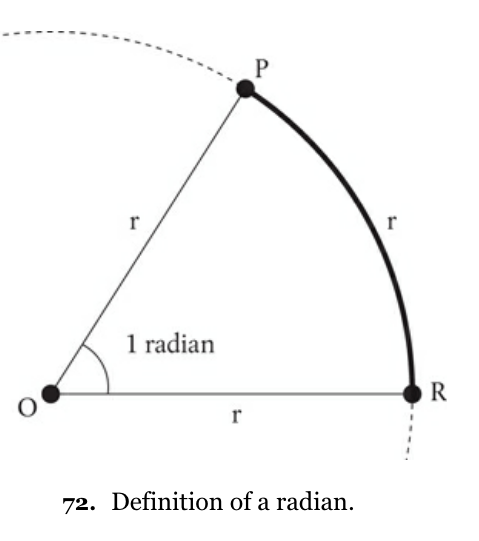
\includegraphics [scale=0.30] {radian.png} \end{center}

We say that the angle $\theta$ is equal to the arc it sweeps out on the circumference, in radians.
\[ s = \theta \]

To convert some more measures of angles in degrees to radians:
\[ 180^\circ = \pi, \ 90^\circ = \frac{\pi}{2} \]
\[ 60^\circ = \frac{\pi}{3}, \ 45^\circ = \frac{\pi}{4}, \ 30^\circ = \frac{\pi}{6} \]

\subsection*{theorem}

In this chapter, we introduce a few more theorems concerning circles, starting with the last of Thales' theorems:

$\circ$  Any angle inscribed in a semicircle is a right angle.

Now, think of three points on the circumference of the circle as forming a triangle. If two points are on a diameter of the circle, the angle formed at any arbitrary but distinct third point is always a right angle.

To prove: $\angle PRQ$ is a right angle.
\begin{center}
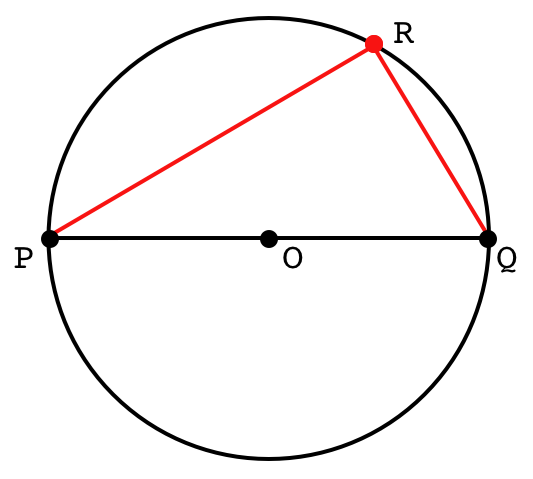
\includegraphics [scale=0.25] {arcs2.png} 
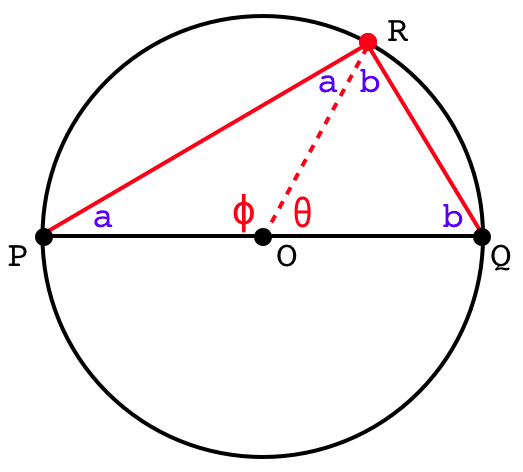
\includegraphics [scale=0.25] {arcs3.png}
\end{center}
Solution:
Draw the radius OR. Notice that $\triangle OPR$ and $\triangle OQR$ are both isosceles.

Label the respective base angles $a$ and $b$. By considering that together the sum of the angles of $\triangle PQR$ can be written:
\[ 2a + 2b  = \pi \]
\[ a + b = \frac{\pi}{2} \]
But this is the measure of $\angle PRQ$.

In addition, the arcs swept out by angles $a$ and $b$ (OPR and OQR on the diameter) clearly add up to $\pi$. This suggests that:

\[ a = \frac{\theta}{2} \]
\[ b = \frac{\phi}{2} \]

Proof:
\[ 2a + 2b = \pi = 2a + \phi \]
\[ \phi = 2b \]

Consider the chord PR and draw the tangent at P.
\begin{center} 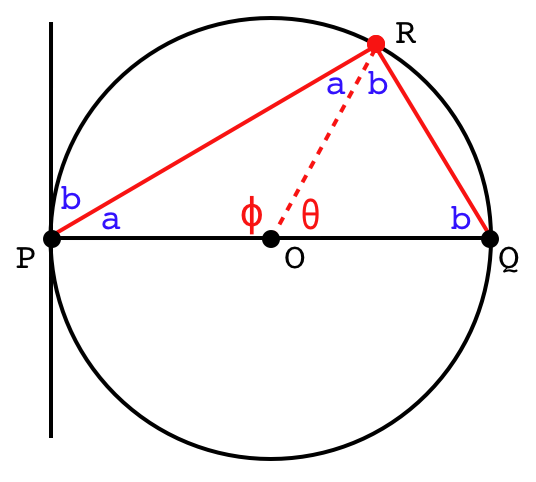
\includegraphics [scale=0.25] {arcs4.png} \end{center}
The arc between the tangent and the chord equals 2b because it is the same arc as cut off by $\angle \ PQR$ (which is $\angle \ b$).

Take a chord of the circle, draw the diameter and the tangent.
The same rule applies to both angles: one between the chord and the diameter, and the second between the chord and the tangent. The arc is twice the measure of the angle.

\subsection*{Generalized arc}

\label{sec:generalized_arc}

Having established these basic facts we can do a bit more.  We will use some of these results later on.

One is to generalize the result for all arcs. The examples so far contain the diameter in some way. Consider the arc swept out by the angle $\theta$ in this figure.
\begin{center} 
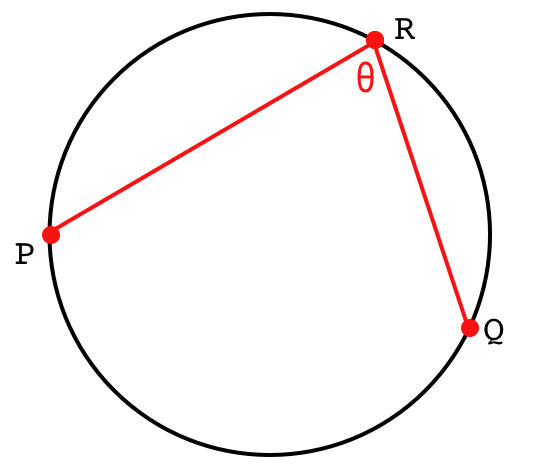
\includegraphics [scale=0.25] {arcs5.png} 
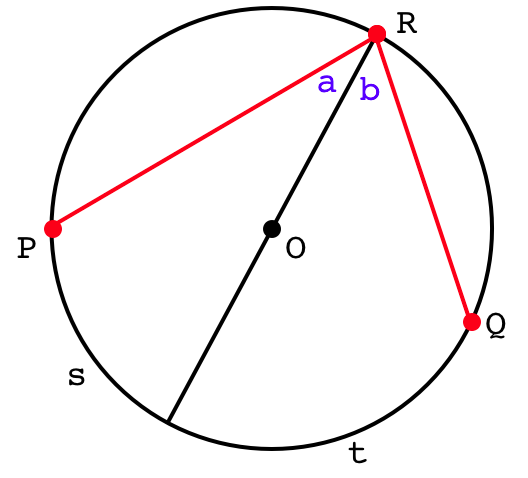
\includegraphics [scale=0.25] {arcs6.png}
\end{center}
We can prove that the measure of the angle $\theta$ is equal to the 1/2 the arc swept out between P and Q. For a simple proof, draw the diameter:
By our previous work:

\[ b = \frac{t}{2} \]
\[ a = \frac{s}{2} \]
\[ \theta = a + b = \frac{s+t}{2} \]

We have proved the theorem for two cases:  where the diameter is one line segment flanking the angle, and where the angle includes the diameter.  However, the theorem is true even if the angle does not include the diameter.
\begin{center} 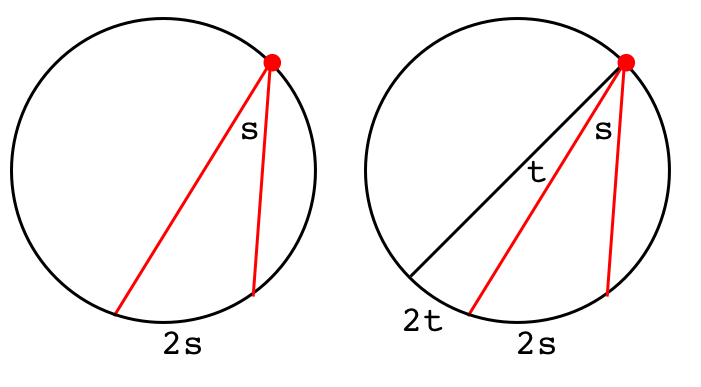
\includegraphics [scale=0.30] {arcs17.png} \end{center}
On the right, draw the diameter.  Notice that we have two arcs which include the diameter:  one with angle $t$ and one with angle $s+t$.  We obtain the generalized arc with angle $s$ by subtraction.

As a corollary, any two angles with vertexes on the circle that cut off the same arc are equal.  In the figure, $s = t$.  Also the triangles are similar triangles.
\begin{center} 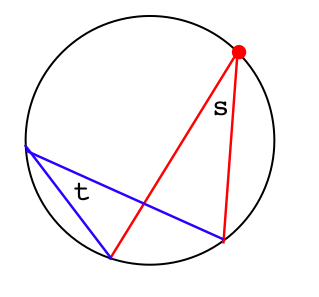
\includegraphics [scale=0.4] {arcs18.png} \end{center}

\subsection*{Intersecting chords}
Given two chords,
to prove:

\[ \theta = 1/2 (s + t) \]

\begin{center} 
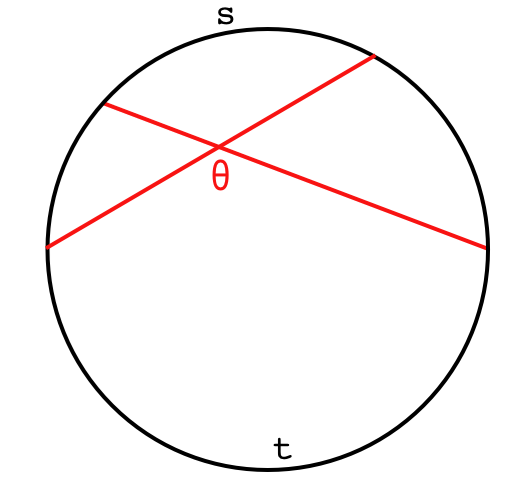
\includegraphics [scale=0.25] {arcs7.png} 
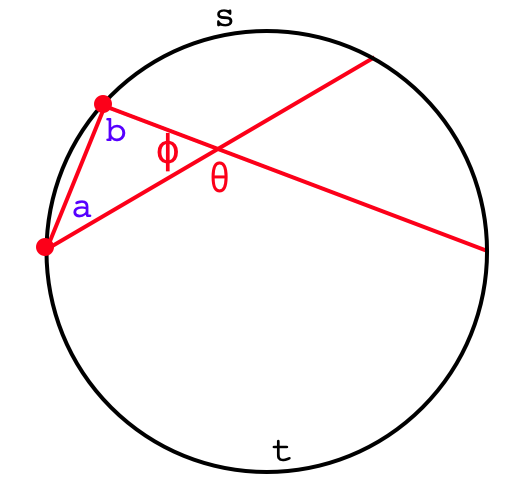
\includegraphics [scale=0.25] {arcs8.png}
\end{center}

$\theta$ is the average of the two arc lengths.
Solution:
Draw a triangle.

\[ a = \frac{s}{2} \]
\[ b = \frac{t}{2} \]
\[ a + b = \theta = \frac{s+t}{2} \]

\subsection*{Tangent and secant}

Rather than having all three points on the circle, one is now outside. We have the same arc swept out by the endpoints ($t$), but the included angle is now smaller, and there is a new small piece of arc length $s$.

\begin{center} 
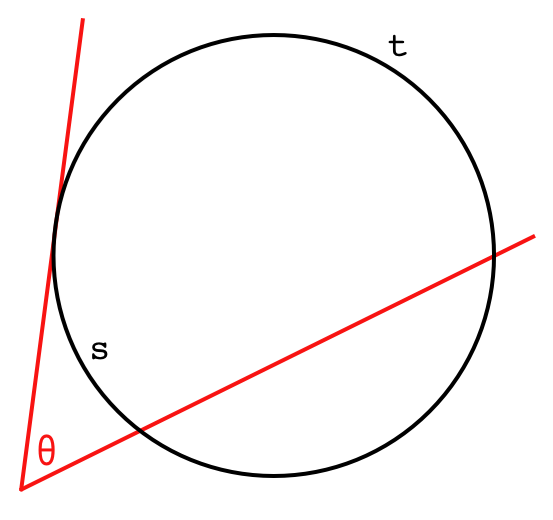
\includegraphics [scale=0.25] {arcs9.png} 
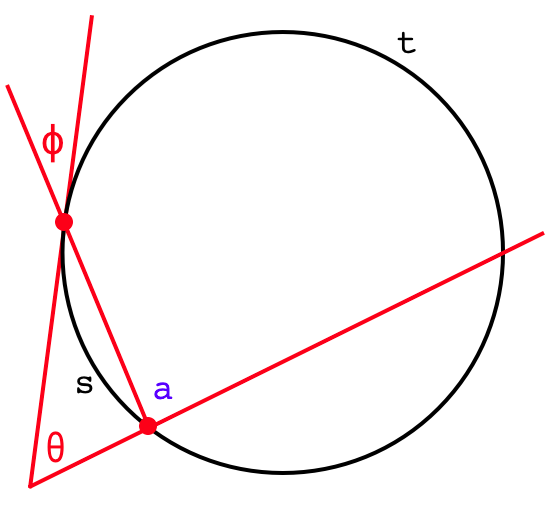
\includegraphics [scale=0.25] {arcs10.png}
\end{center}

To prove:

\[ \theta = \frac{t-s}{2} \]

Solution:
Draw the triangle.
By our previous work (and supplementary angles):

\[ \phi = \frac{s}{2} \]
\[ a = \frac{t}{2} \]

by supplementary angles:

\[ \theta + \phi = a \]
\[ \theta = \frac{t}{2} - \frac{s}{2} \]
\[ = \frac{t-s}{2} \]

\subsection*{Chord segments}

Finally, there is a simple algebraic relationship between chord segments. Draw two chords of the circle and label the lengths of the segments as shown (note: $s$ and $t$ do not refer to arcs any more).

\begin{center} 
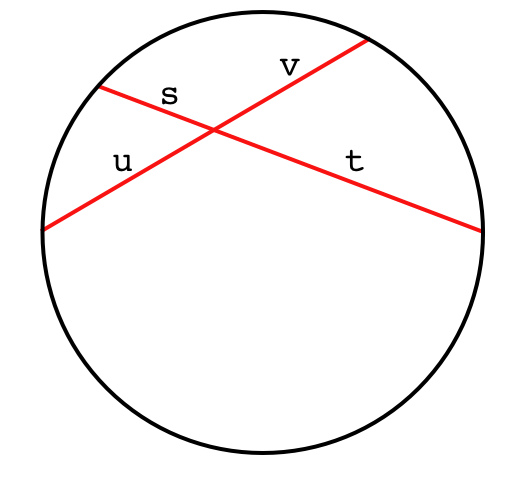
\includegraphics [scale=0.25] {arcs15.png} 
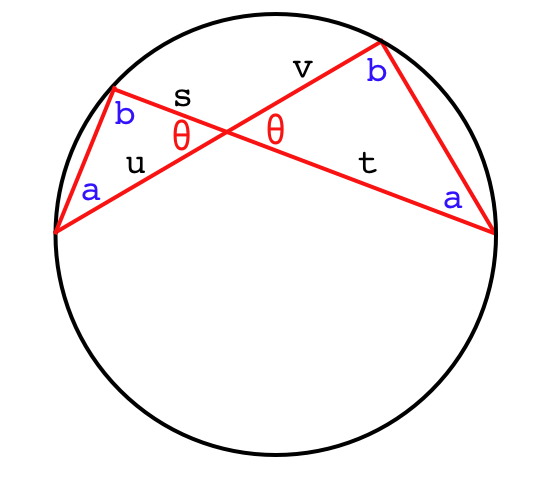
\includegraphics [scale=0.25] {arcs16.png}
\end{center}
Draw the two triangles.
Notice that the two angles labeled $a$ are equal because they sweep out the same arc of the circle, and similarly for the two angles labeled $b$. By similar triangles:

\[ s/u = v/t \]
\[ st = uv \]

\end{document}